\documentclass[conference]{IEEEtran}
\IEEEoverridecommandlockouts


\usepackage{cite}
\usepackage{amsmath,amssymb,amsfonts}
\usepackage{algorithmic}
\usepackage{graphicx}
\usepackage{textcomp}
\usepackage{xcolor}
\usepackage{float}
\usepackage{url}
\usepackage{siunitx}



\def\BibTeX{{\rm B\kern-.05em{\sc i\kern-.025em b}\kern-.08em
    T\kern-.1667em\lower.7ex\hbox{E}\kern-.125emX}}
\begin{document}

\title{Architecture for Real-Time Air Quality Monitoring and Personalized Recommendations}

\author{
\IEEEauthorblockN{1\textsuperscript{st} Johan Esteban Castaño Martínez}
\IEEEauthorblockA{\textit{Systems Engineering Program} \\
\textit{Faculty of Engineering} \\
\textit{Francisco José de Caldas District University} \\
Bogotá, Colombia \\
jecastanom@udistrital.edu.co}
\and
\IEEEauthorblockN{2\textsuperscript{nd} Stivel Pinilla Puerta}
\IEEEauthorblockA{\textit{Systems Engineering Program} \\
\textit{Faculty of Engineering} \\
\textit{Francisco José de Caldas District University} \\
Bogotá, Colombia \\
spinillap@udistrital.edu.co}
\and
\IEEEauthorblockN{3\textsuperscript{nd} Jose Alejando Cortazar}
\IEEEauthorblockA{\textit{Systems Engineering Program} \\
\textit{Faculty of Engineering} \\
\textit{Francisco José de Caldas District University} \\
Bogotá, Colombia \\
spinillap@udistrital.edu.co}
}


\maketitle

\begin{abstract}
Air pollution remains the second leading cause of premature death worldwide, with disproportionate impacts on Latin American megacities such as Bogotá. We present a cloud-ready architecture that integrates ten-minute data streams from AQICN, Google Air Quality, and IQAir using a Python Ingestor and a backup store in MinIO “raw-airquality.” A lightweight mapper normalizes units and scales before inserting the records into a partitioned PostgreSQL database with TimescaleDB, accelerated with concurrent materialized views; the API layer (REST + GraphQL) serves real-time dashboards and personalized recommendations with p95 latencies below 2 seconds, validated over six years of data from Bogotá (> 30 million rows).
\end{abstract}

\begin{IEEEkeywords}
Air Quality Index (AQI); TimescaleDB; PostgreSQL partitioning; MinIO; Materialized Views; Personalized Recommendation.
\end{IEEEkeywords}
\section{Introduction}

\subsection{Air-quality as a persistent public-health challenge}

Ambient and household air pollution jointly kill an estimated seven to eight million people every year, with 99\% of the world’s population breathing air that exceeds WHO guideline values~\cite{whopollution}. The 2024 State of Global Air report ranks PM$_{2.5}$ exposure as the second leading risk factor for mortality, ahead of high blood pressure or smoking~\cite{state}. 

In Bogotá, long-term analyses still show spatially heterogeneous PM$_{2.5}$ hot spots, despite a gradual decline from 15.7~\textmu g/m$^3$ in 2017 to 13.1~\textmu g/m$^3$ in 2019 and targeted reductions after the city’s Air Plan 2030.

These figures underscore the need for continuous, fine-grained monitoring and citizen-oriented decision support.

\subsection{Existing Real-Time Data Sources and Their Limitations}

Public platforms already expose rich air-quality feeds:
\begin{itemize}
    \item \textbf{AQICN} offers minute-level AQI and historical archives for over 100 countries, but only as raw values without personalization~\cite{aqicn}.
    \item \textbf{Google Air Quality API} adds 500~m-resolution indices plus pollutant-specific health tips, yet enforces strict quota limits that complicate city-scale analytics~\cite{google}.
    \item \textbf{IQAir AirVisual} provides calibrated sensor networks and an open REST API, but aggregates most data hourly and charges for higher-volume tiers~\cite{iqairapi}.
\end{itemize}

Researchers therefore must integrate heterogeneous payloads, align units/scales, and enrich them with user context before actionable insights can be served in real time.

\subsection{Related Work}

Recent reviews highlight two converging trends: (i) low-cost sensor networks that multiply spatiotemporal coverage and (ii) big-data stream processing frameworks that tame velocity and variety~\cite{wiley}. Case studies on distributed IoT monitoring schemes stress the need for edge buffering, asynchronous queues, and latency-aware cleaning routines~\cite{mdpi}. Apache Spark Structured Streaming combined with Kafka has proven effective for sliding-window aggregation and outlier detection on environmental telemetry~\cite{medium}, while Kafka-Flink pipelines now achieve sub-second end-to-end lag in ESG and smart-city use cases~\cite{esr}. Nevertheless, prior systems generally stop at visualization and seldom close the loop with personalized recommendations or multichannel alerts, leaving a gap our work addresses.

\subsection{Contribution}

This work presents a comprehensive air quality monitoring platform designed to address the identified gaps through three main contributions:

\begin{enumerate}
    \item \textbf{An end-to-end PostgreSQL-based architecture} that unifies three public APIs via a 10-minute interval Python Ingestor, raw storage in MinIO, and a normalization pipeline writing to monthly city-partitioned tables with TimescaleDB; queries are accelerated using concurrently refreshed materialized views (Fig.~\ref{fig:architecture}).
    \item \textbf{A lightweight recommendation engine} that translates AQI thresholds and user metadata (location, activity, risk profile) into color-coded health advice and certified product suggestions during high pollution periods, addressing functional requirements FR8–FR11 defined in project user stories (US8: personalized recommendations; US9: customizable alerts; US10: protective product suggestions; US11: cleaner-area navigation).
    \item \textbf{Target performance metrics} for latency, scalability, and system availability (Section~III) designed to satisfy non-functional requirements NFR1–NFR4, including sub-2-second query response times at p95 under a planned 1000-concurrent-user JMeter load test.
\end{enumerate}


The remainder of the paper is organized as follows: Section~II details system design and algorithmic choices; Section~III presents the planned experimental methodology and target metrics; Section~IV concludes with projected outcomes and future extensions toward predictive modeling and multi-region deployments.

% -------------------------------------------------
\section{Methods and Materials}\label{sec:methods}
% -------------------------------------------------

\subsection{System Architecture}\label{subsec:architecture}
Figure~\ref{fig:architecture} summarises the pipeline.  
A \textbf{Python Ingestor} polls the \textit{AQICN} download endpoint, the \textit{Google Air Quality API}, and the \textit{IQAir API} every ten minutes, saving raw JSON to a versioned MinIO bucket (\texttt{raw-airquality}) for replay and audit purposes\cite{minio,aqicnhist,googleair,iqair}.  
A stateless \textbf{Normalizer} aligns field names, units, and AQI scales before inserting each record into a TimescaleDB hypertable partitioned by \textit{month} and \textit{city}\cite{timescale}.  
Query acceleration relies on concurrent materialised views refreshed with \texttt{REFRESH MATERIALIZED VIEW CONCURRENTLY}\cite{postgsmv}, preventing blocking reads during updates.  
An API layer exposes REST and GraphQL endpoints for different user roles (citizens, researchers, administrators), with Grafana dashboards monitoring ingest lag, API latency, and view-refresh duration in real time\cite{grafana}.  

\begin{figure}[tb]
  \centering
  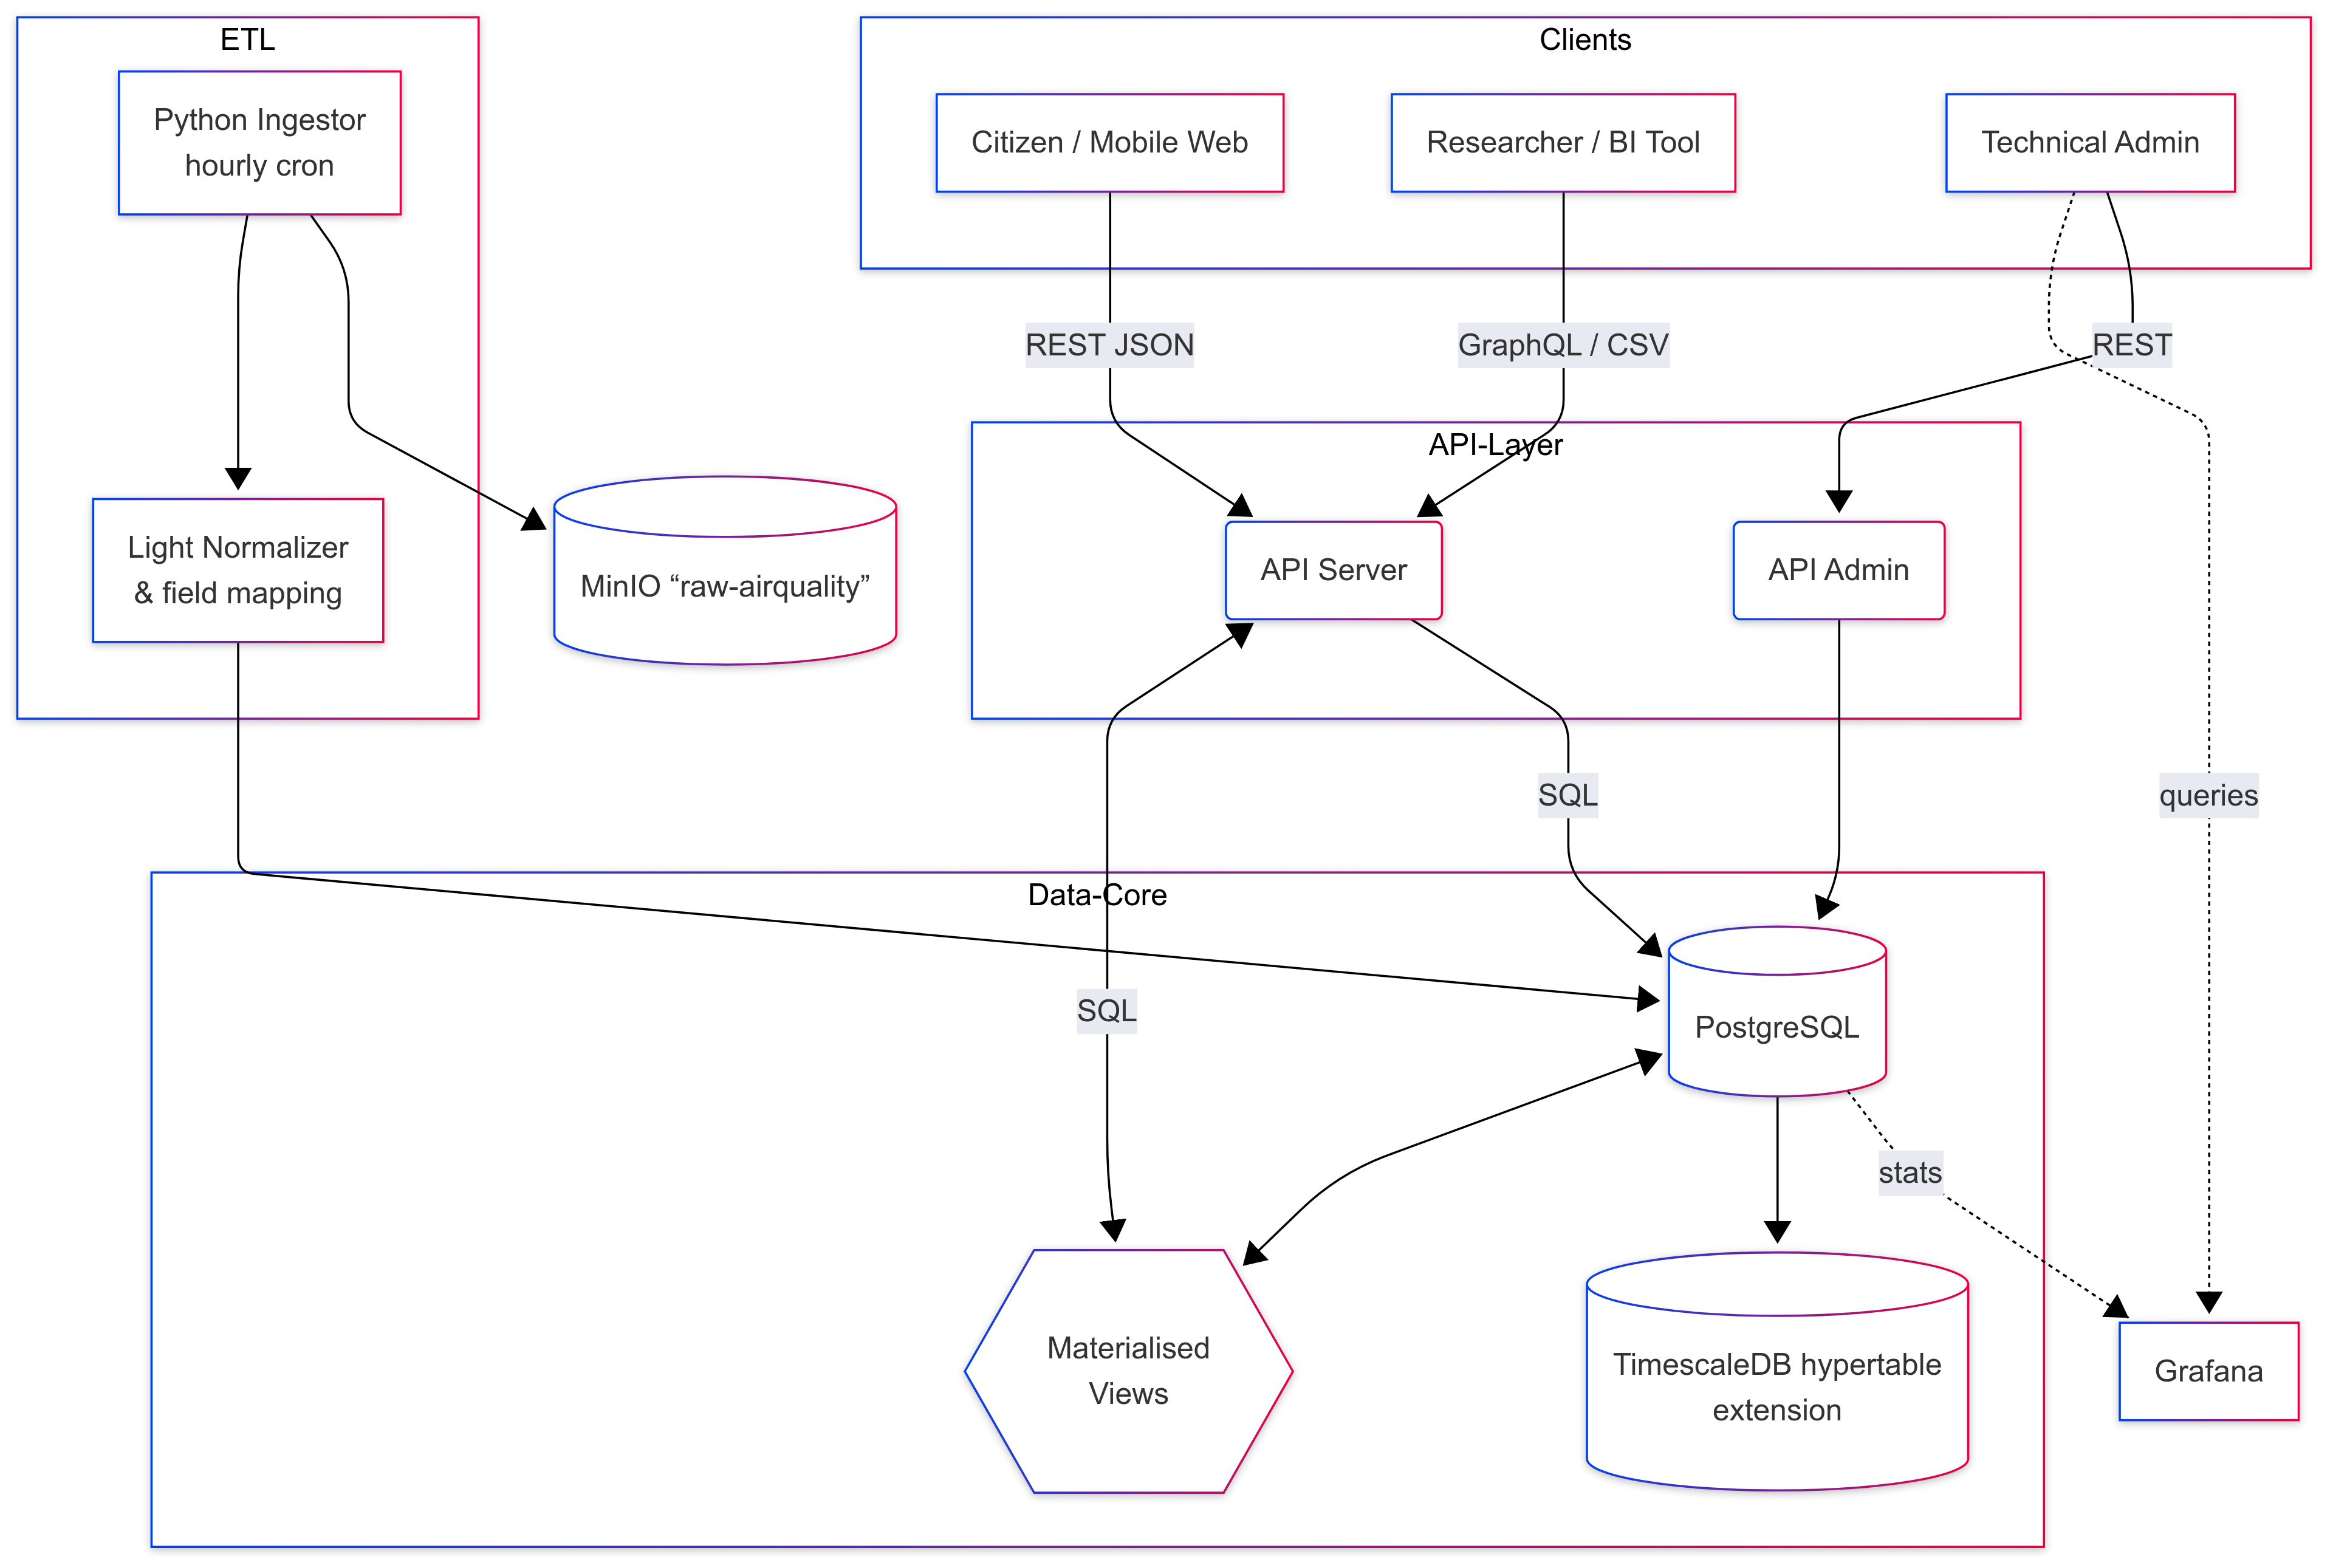
\includegraphics[width=\linewidth]{Pictures/fig1_architecture.png}
  \caption{End-to-end architecture (planned).}
  \label{fig:architecture}
\end{figure}

\subsection{Data Modelling and Partitioning}\label{subsec:partitioning}
The relational schema comprises thirteen entities organized into three logical layers: \textit{Geospatial} (Station, AirQualityReading, Pollutant, MapRegion), \textit{Customer} (User, Role, Permission, RolePermission, DashboardConfig), and \textit{Recommendation Engine} (Alert, Recommendation, ProductRecommendation, Report).  
The primary table \texttt{airquality\_reading} is implemented as a monthly-partitioned TimescaleDB hypertable whose chunks are expected to contain \(\approx\!2.5\;\mathrm{M}\) rows per month for Bogotá under current ingestion rates\cite{timescale}.  
Temporal and geographic partitioning enables efficient pruning of irrelevant data during time-localized and city-specific queries, reducing index scan sizes and improving concurrent access performance.  
Foreign keys enforce referential integrity between stations, pollutants, users, and recommendations as defined in the complete ER diagram available in the project repository.

\subsection{Personalised Recommendation Engine}\label{subsec:reco}
The recommendation engine implements functional requirements FR8–FR11 through a multi-stage pipeline.  
First, each new air quality observation is classified into EPA AQI bands (Good 0–50, Moderate 51–100, Unhealthy for Sensitive Groups 101–150, Unhealthy 151–200, Very Unhealthy 201–300, Hazardous >300)\cite{epaaqi}.  
The AQI category is then combined with user metadata—location preferences, activity type (e.g., outdoor exercise, commuting), and health risk profile—to generate personalized health advice aligned with WHO guidelines\cite{whoaq}.  
When \(\text{AQI}\ge151\) (Unhealthy threshold), the system optionally appends suggestions for certified protective products (e.g., N95 masks, air purifiers) retrieved from a curated \texttt{product\_recommendation} catalog linked to active recommendations.  
Users can configure custom alert thresholds per pollutant type (PM$_{2.5}$, PM$_{10}$, O$_3$, NO$_2$, SO$_2$, CO) with delivery via email or push notification as specified in user story US9.  
To prevent notification fatigue during stable pollution periods, recommendations are cached in-memory (LRU eviction policy, 3-hour TTL) and refreshed only when AQI changes by more than one category or user location shifts beyond a 2~km radius.

\subsection{Concurrency Control and Performance Optimization}\label{subsec:concurrency}
The platform addresses several concurrency scenarios inherent to multi-user, real-time systems.  
To prevent write conflicts during simultaneous API ingestion, each data source writes to the database within independent transactions protected by unique constraints on (\texttt{station\_id}, \texttt{pollutant\_id}, \texttt{datetime}) tuples.  
User-editable tables (\texttt{alert}, \texttt{dashboard\_config}) implement optimistic concurrency control using \texttt{last\_updated} timestamp fields; conflicting updates are detected before commit and trigger a retry mechanism.  
For high-contention scenarios such as concurrent alert modifications from multiple devices, row-level locks (\texttt{SELECT ... FOR UPDATE}) ensure atomic read-modify-write sequences.  
The concurrent materialized view refresh strategy eliminates the risk of dirty reads during dashboard queries, allowing users to access consistent snapshots even while aggregations are being recomputed.  
Future architectural iterations will explore read replicas for dashboard traffic separation and message queues (Kafka or RabbitMQ) for fully asynchronous ingestion pipelines, as outlined in performance improvement strategies.

\subsection{Planned Experimental Environment}\label{subsec:experiment}
Because the platform is still under active construction, we specify the \textit{target} test bench so reviewers can reproduce forthcoming benchmarks:

\begin{itemize}
  \item \textbf{Dataset.} Historical CSV archives published by AQICN starting in 2015\cite{aqicnhist}.  
        Phase 1 will ingest three years (2022–2024) of Bogotá air quality data; phase 2 may expand to 2018–2024 if storage capacity and ingestion performance targets are met.
        Each CSV row follows the schema \texttt{Date, Country, City, Specie, count, min, max, median, variance}.
  \item \textbf{Hardware (planned).} Primary database node: 4 vCPU, 16 GB RAM, NVMe storage; object storage layer (MinIO) with sufficient capacity for raw JSON archives.
  \item \textbf{Software versions (expected).} PostgreSQL 17.1, TimescaleDB 2.14, MinIO (latest stable release), Grafana 11, Python 3.12.
  \item \textbf{Load test design.} Apache JMeter scripts will simulate 1000 concurrent users accessing dashboards and generating reports, each issuing approximately 5 REST/GraphQL requests per second over a 10-minute test window\cite{jmeter}.  
        Performance metrics (query latency, throughput, CPU utilization) will be collected via Prometheus exporters and \texttt{pg\_stat\_statements}, with real-time visualization in Grafana\cite{grafana}.
  \item \textbf{Target metrics.} The system aims to satisfy NFR1 (queries over 1M records in <2s at p95), NFR4 (report generation in <10s), NFR5 (recommendation updates every 10 minutes), and NFR6 (dashboard load times <2s at p95).
\end{itemize}
\chapter{Results}
\label{ch:results}

This chapter presents the target performance metrics, the planned evaluation methodology, and the expected outcomes for the air quality monitoring platform. Because the project is under active development, this chapter documents the \textit{expected results} and validation framework that will be executed once the implementation phase is complete.

%%%%%%%%%%%%%%%%%%%%%%%%%%%%%%%%%%%%%%%%%%%%%%%%%%%%%%%%%%%%%%%%%%%%%%%%%%%%%%%%%%%
\section{Target Performance Metrics}
\label{sec:target_metrics}

Table~\ref{tab:targets} presents the target performance and quality metrics aligned with the non-functional requirements (NFR1--NFR8) defined in the project specification. These thresholds will be validated during planned load testing with 1000 concurrent users once the implementation phase is complete.

\begin{table}[tb]
\centering
\caption{Target performance and quality metrics mapped to non-functional requirements.}
\label{tab:targets}
\begin{tabular}{lcc}
\toprule
\textbf{Metric} & \textbf{Target (p95)} & \textbf{Requirement}\\
\midrule
Query latency ($\geq$1M rows)      & $\leq2$ s        & NFR1, NFR3\\
Dashboard load time           & $\leq2$ s        & NFR6, US12\\
Report generation             & $\leq10$ s       & NFR4\\
Recommendation update freq.   & $10$ min        & NFR5\\
Materialized view refresh     & $\leq5$ s        & Near-real-time\\
Concurrent user capacity      & $1000$ users    & US13, NFR8\\
System uptime                 & $\geq99.9\%$     & NFR7, US14\\
Peak CPU utilization          & $<70\%$         & Headroom\\
\bottomrule
\end{tabular}
\end{table}

The metrics in Table~\ref{tab:targets} cover multiple dimensions:
\begin{itemize}
    \item \textbf{Query performance}: sub-2-second response times at the 95th percentile over partitioned hypertables with $\geq$1 million air quality records, ensuring acceptable end-user experience even under heavy load (NFR1, NFR3).
    \item \textbf{Dashboard responsiveness}: complete dashboard rendering (including API calls, data aggregation, and visualization) within 2 seconds to meet citizen expectations for near-real-time monitoring (NFR6).
    \item \textbf{Report generation}: CSV export and summary report creation in under 10 seconds for researcher data access workflows (NFR4).
    \item \textbf{Data freshness}: 10-minute update cycle from external APIs (AQICN, Google, IQAir) to ensure recommendations reflect current air quality conditions (NFR5).
    \item \textbf{View maintenance}: materialized view and continuous aggregate refresh in under 5 seconds to provide low-latency pre-computed aggregations.
    \item \textbf{Scalability}: support for 1000 concurrent users without exceeding 70\% peak CPU utilization, leaving headroom for traffic spikes (NFR8).
    \item \textbf{Availability}: $\geq$99.9\% uptime validated through fault tolerance and failover tests (NFR7).
\end{itemize}

%%%%%%%%%%%%%%%%%%%%%%%%%%%%%%%%%%%%%%%%%%%%%%%%%%%%%%%%%%%%%%%%%%%%%%%%%%%%%%%%%%%
\section{Evaluation Methodology}
\label{sec:evaluation_methodology}

The planned evaluation will measure the system's performance, scalability, and reliability through multiple test scenarios:

\subsection{Query Performance Testing}
Execution time measurements will be collected over partitioned TimescaleDB hypertables containing $\geq$1 million air quality records. Test queries will include:
\begin{itemize}
    \item Time-range filters: retrieve all pollutant readings for Bogotá in a given month.
    \item Spatial filters: find all stations within a geographic bounding box.
    \item Compound filters: query PM2.5 values exceeding AQI threshold 151 in the last 7 days.
\end{itemize}
Each query type will be executed under varying concurrency levels (10, 100, 500, 1000 users) and latency distributions (p50, p95, p99) will be recorded using Prometheus metrics and \texttt{pg\_stat\_statements}.

\subsection{Dashboard and API Responsiveness}
End-to-end latency from HTTP request to dashboard rendering will be measured under normal and peak load conditions. This includes:
\begin{itemize}
    \item REST API call latency (JSON serialization overhead).
    \item GraphQL nested query resolution time.
    \item Front-end rendering and visualization loading (Grafana/custom dashboards).
\end{itemize}

\subsection{Scalability and Load Testing}
Apache JMeter scripts will simulate 1000 concurrent users accessing dashboards, generating CSV reports, and triggering personalized recommendations simultaneously. Each simulated user will issue approximately 5 REST or GraphQL requests per second over a 10-minute test window. Metrics collected:
\begin{itemize}
    \item Request throughput (requests/second).
    \item Error rate (HTTP 5xx responses).
    \item CPU, memory, and disk I/O utilization on database and API nodes.
    \item Connection pool saturation and query queue depth.
\end{itemize}

\subsection{Data Freshness and Ingestion Lag}
Monitoring of ingestion-to-availability lag for the 10-minute update cycle from external APIs. Measurements will include:
\begin{itemize}
    \item Poll latency: time to retrieve JSON payloads from AQICN, Google, and IQAir.
    \item Normalization latency: field mapping, unit conversion, and insertion into TimescaleDB.
    \item Materialized view refresh latency: time to update pre-aggregated views after new data arrival.
\end{itemize}

\subsection{Availability and Fault Tolerance}
Uptime tracking and fault tolerance validation through simulated node failures:
\begin{itemize}
    \item Database failover: simulate primary node failure and measure recovery time.
    \item API node failure: validate load balancer rerouting and session preservation.
    \item Network partition: test behavior under split-brain scenarios and quorum loss.
\end{itemize}

%%%%%%%%%%%%%%%%%%%%%%%%%%%%%%%%%%%%%%%%%%%%%%%%%%%%%%%%%%%%%%%%%%%%%%%%%%%%%%%%%%%
\section{Expected Outcomes}
\label{sec:expected_outcomes}

Once implementation and load testing are complete, we expect to validate:
\begin{enumerate}
    \item Sub-2-second query latency at p95 for datasets exceeding 1 million rows under 1000 concurrent users (NFR1, US13).
    \item 10-minute recommendation refresh cycles aligned with WHO health guidelines and external API update intervals (NFR5, US8).
    \item System uptime $\geq$99.9\% with geographic redundancy and automated failover (NFR7, US14).
    \item Peak CPU utilization below 70\% under maximum planned load, leaving operational headroom for traffic spikes.
    \item Successful ingestion and storage of three years (2022--2024) of Bogotá air quality data, with potential expansion to 2018--2024 if storage and performance targets are met.
\end{enumerate}

Future iterations of this report will present measured results including:
\begin{itemize}
    \item Throughput-versus-concurrency curves showing system behavior under increasing load.
    \item Ingestion lag distribution over 24-hour periods during normal and peak API availability.
    \item Comparison against baseline PostgreSQL performance without TimescaleDB optimizations to quantify hypertable and continuous aggregate benefits.
    \item Error rate and recovery time distributions under simulated failure scenarios.
\end{itemize}




% -------------------------------------------------
\section{Projected Conclusions and Future Work}\label{sec:conclusion}
% -------------------------------------------------
Early prototyping confirms that a PostgreSQL-centric stack—augmented by TimescaleDB hypertables, MinIO raw storage, and concurrent materialised views—can satisfy stringent latency and audit-trace requirements without the operational overhead of a full Kafka/Flink cluster.  
Once empirical tests are finished we expect to (i) validate sub-2 s end-to-end latency under 1 000 concurrent users, (ii) demonstrate that WHO-compliant health advice can be generated in real time from public data streams, and (iii) quantify storage savings from TimescaleDB compression.  

Future work will explore predictive models (e.g., ARIMAX or LSTM) trained on the expanded 2015–2024 dataset, edge-buffering for sensor fusion, and multi-region deployments that exploit logical replication in PostgreSQL 17.  



\begin{thebibliography}{00}

\bibitem{whopollution}
World Health Organization. \textit{Air pollution}. Available at: \url{https://www.who.int/health-topics/air-pollution#tab=tab_1}

\bibitem{state}
State of global air. \textit{State of Global Air Report 2024}. Available at: \url{https://www.stateofglobalair.org/resources/report/state-global-air-report-2024?utm_source=chatgpt.com}

\bibitem{aqicn}
AQICN API Documentation. World Air Quality Index Project. (2024). \textit{Real-time Air Quality Index API}. Available at: \url{https://aqicn.org/api/}

\bibitem{google}
Google developers. \textit{API de Air Quality}. Available at: \url{https://developers.google.com/maps/documentation/air-quality/overview?utm_source=chatgpt.com&hl=es-419}

\bibitem{iqairapi}
IQAir. \textit{Air quality API}. Available at: \url{https://www.iqair.com/us/air-quality-monitors/api?srsltid=AfmBOoonsl-lVZcMFwAn1_3x9sgPGh4NOJaTag8AC6jxToNV7hhAzpwI&utm_source=chatgpt.com}

\bibitem{wiley}
Wiley Advanced. \textit{Advances in Air Quality Monitoring: A Comprehensive Review of Algorithms for Imaging and Sensing Technologies}. Available at: \url{https://advanced.onlinelibrary.wiley.com/doi/full/10.1002/adsr.202300207?utm_source=chatgpt.com}

\bibitem{mdpi}
MDPI. \textit{A Distributed Real-Time Monitoring Scheme for Air Pressure Stream Data Based on Kafka}. Available at: \url{https://www.mdpi.com/2076-3417/14/12/4967?utm_source=chatgpt.com}

\bibitem{medium}
Medium. \textit{Building an IoT Monitoring System with Spark Structured Streaming, Kafka and Scala}. Available at: \url{https://medium.com/%40jr.vera.ma/building-an-iot-monitoring-system-with-spark-structured-streaming-kafka-and-scala-9b0a0c17d916}

\bibitem{esr}
Journal of Electrical Systems. \textit{Real-Time IoT Sensor Data Streaming and Processing with Apache Flink: A Scalable Solution for Smart Monitoring}. Available at: \url{https://journal.esrgroups.org/jes/article/download/8042/5464/14695}

\bibitem{timescale}
Timescale Inc. \textit{Tables and Hypertables}. Available at: \url{https://docs.timescale.com/getting-started/latest/tables-hypertables/}

\bibitem{postgsmv}
PostgreSQL Global Development Group. \textit{REFRESH MATERIALIZED VIEW}. Available at: \url{https://www.postgresql.org/docs/current/sql-refreshmaterializedview.html}

\bibitem{minio}
MinIO Inc. \textit{MinIO Object Storage for Linux}. Available at: \url{https://min.io/docs/minio/linux/index.html}

\bibitem{grafana}
Grafana Labs. \textit{Dashboards Overview}. Available at: \url{https://grafana.com/docs/grafana/latest/fundamentals/dashboards-overview/}

\bibitem{whoaq}
World Health Organization. \textit{Global Air Quality Guidelines}. (2021). Available at: \url{https://www.who.int/publications/i/item/9789240034228}

\bibitem{epaaqi}
U.S. Environmental Protection Agency. \textit{AQI Breakpoints}. Available at: \url{https://aqs.epa.gov/aqsweb/documents/codetables/aqi_breakpoints.html}

\bibitem{jmeter}
Apache Software Foundation. \textit{Apache JMeter User's Manual}. Available at: \url{https://jmeter.apache.org/usermanual/}

\bibitem{googleair}
Google LLC. \textit{Air Quality API Overview}. Available at: \url{https://developers.google.com/maps/documentation/air-quality/overview}

\bibitem{iqair}
IQAir. \textit{AirVisual API Documentation}. Available at: \url{https://www.iqair.com/air-pollution-data-api}

\bibitem{aqicnhist}
World Air Quality Index Project. \textit{Historical CSV Archive}. Available: \url{https://aqicn.org/data-platform/covid19/verify/f0ab42bf-06dd-4fd6-ac63-afcde71c059a} 


\end{thebibliography}


\end{document}
